\lecture{1-1}{28. Januar 2025}{Introduction and the Laws of thermodynamics}

\section{Introduction to thermodynamics}

\begin{definition}[Thermodynamics]
  \textit{Thermodynamics} comes from greek \textit{thermos} meaning \textit{heat} and \textit{dynamics} meaning \textit{in motion}. All in all \textit{thermodynamics} is the study of \textit{heat in motion}.
\end{definition}
An example of a simple thermodynamic cycle is the Rankine cycle in \autoref{fig:F1_1}. The Rankine cycle is often mentioned as the simplest thermodynamic cycle.

\begin{figure} [ht]
  \centering
  \caption{A Rankine cycle}
  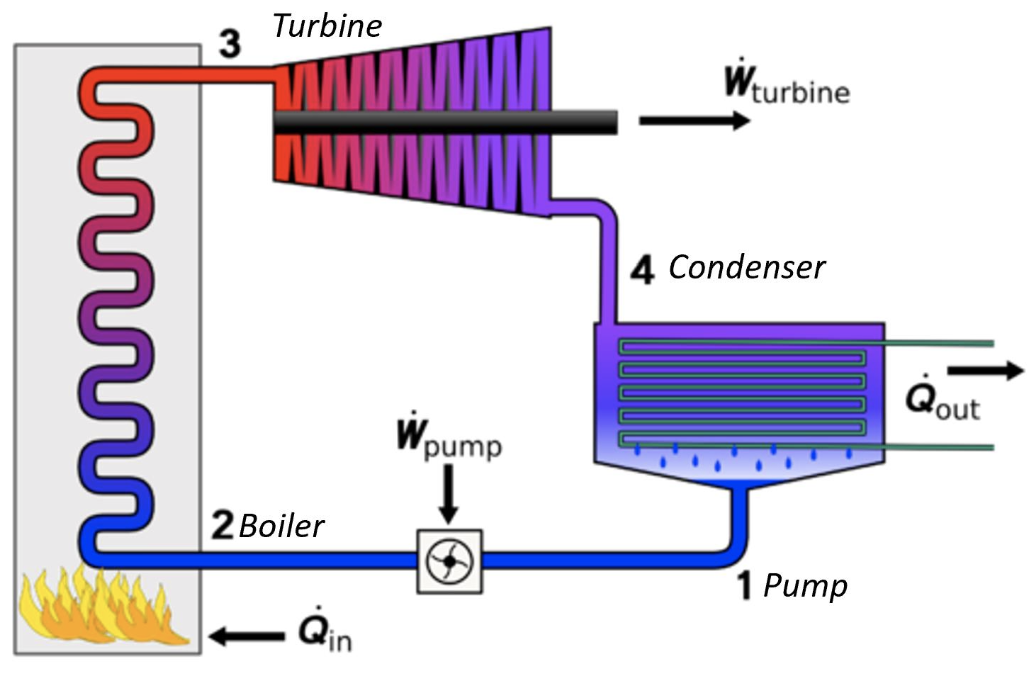
\includegraphics[width=0.5\linewidth]{./figures/F1_1.png}
  \label{fig:F1_1}
\end{figure}


\subsection{General heat engines}
\begin{figure} [ht]
  \centering
  \caption{A general heat engine}
  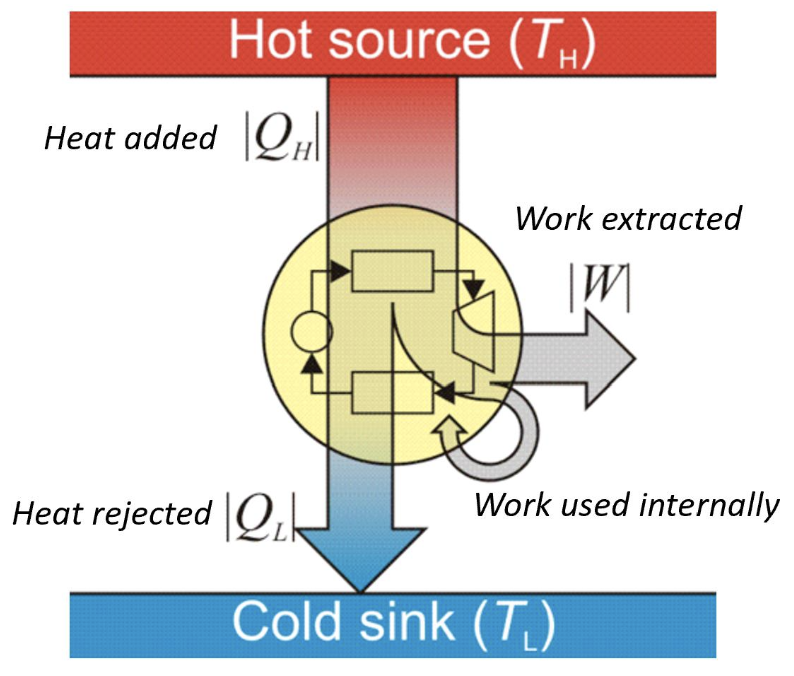
\includegraphics[width=0.5\linewidth]{./figures/F1_2.png}
  \label{fig:F1_2}
\end{figure}
A heat engine is an engine that extracts heat from a hot source and converts (some of) this heat into work and rejects the rest into a cold sink. This is shown in \autoref{fig:F1_2}. The physicist \textit{Sadi Carnot} has shown that the ideal efficiency (called the \textit{Carnot-efficiency}) of a heat engine is given by
\[ 
\eta_{\text{max}} = 1 - \frac{T_c}{T_h}
\]
Where $T_c$ is the temperature of the cold sink and $T_h$ is the temperature of the hot source. The Carnot-efficiency is the \textit{theoretical} maximal efficiency of any heat engine. Common heat engines have an efficiency about half as big as the Carnot efficiency.

\begin{eks}[Carnot-efficiency of a heat engine]
  We want to calculate the Carnot-efficiency of a heat engine working between the temperatures of $T_h = \qty{1000}{\celsius}$ and $T_c = \qty{0}{\celsius}$.
  \bigbreak
  The formulation of Carnots law is
  \[ 
  \eta_{\mathrm{max}} = 1 - \frac{T_c}{T_h} = 1 - \frac{\qty{27,153}{K}}{\qty{1273,15}{K}} = \num{0,786}  
  .\]
\end{eks}

\subsection{The laws of thermodynamics}
Three main rules have been made for the field of thermodynamics. These are

\begin{sæt}[1st law of thermodynamics]
  The 1st law of thermodynamics states that energy is always conserved and can be formulated as: \textit{All energy is conserved, only its form can be changed}. Related to the 1st law of thermodynamics is the fact that mass is also conserved.
\end{sæt}

\begin{sæt}[2nd law of thermodynamics]
  The second law of thermodynamics states that energy only moves spontaneously from a hot area to a cold area. 
\end{sæt}

\begin{sæt}[3rd law of thermodynamics]
  The third law of thermodynamics states that the entropy of a pure crystalline solid with a temperature of \qty{0}{K} has an entropy of 0.
\end{sæt}


\subsection{Types of thermodynamical systems}
\begin{definition}[Solid boundary]
  A solid system boundary is any boundary of a system that cannot change size or shape.
\end{definition}

\begin{definition}[Displaceable boundary]
  A displaceable system boundary is any boundary of a system that is not fixed and thus is free to expand, shrink or change its shape in another way.
\end{definition}

\begin{definition}[Closed system]
  A closed system is any system that does not allow transfer of mass over its boundary. Energy is however able to move over the boundary of a closed system. 
\end{definition}

\begin{definition}[Open system]
  An open system is any system that allows transfer of mass and energy across its boundary.
\end{definition}

\begin{figure}[ht]
  \centering
  \incfig[0.25]{F1_3}
  \caption{Drawing showing the system boundaries of a kettle (the kettle, heating element and air above water is not included in the system.)}
  \label{fig:F1_3}
\end{figure}

\begin{eks}[The system boundary and energy balance for an electric kettle]
  On \autoref{fig:F1_3} a simplified drawing of a kettle can be seen. It is evident, that the kettle is able to let mass (steam) pass through its opening and therefore it seems obvious it should be an open system. However as long as the temperature does not reach \qty{100}{\celsius} then it is a reasonable approximation to see the system as closed. We now the specific heat formula to be
  \[ 
  E = m \cdot c_p \cdot \Delta T
  .\]
\end{eks}

\begin{definition}[Adiabatic system]
  An adiabatic system is any system that does not allow transfer of heat over the system boundaries.
\end{definition}

\begin{figure}[ht]
  \centering
  \incfig[0.5]{F1_4}
  \caption{Drawing of the mixing problem described underneath.}
  \label{fig:F1_4}
\end{figure}

\begin{eks} [Temperature of water after mixing]
  \qty{1}{L} of water with a temperature of \qty{20}{\celsius} is mixed with an equal amount of water with a temperature of \qty{40}{\celsius}. We want to determine the temperature at the end.
  \bigbreak
  On \autoref{fig:F1_4} a drawing of the system is shown. We can remember the formulation of the formula for specific heat to be
  \[ 
  E = m \cdot c_p \cdot \Delta T
  .\]
  If we assume that no energy is lost during the mixing then it must be true that the total amount of energy is the same before mixing and after mixing (1st law of thermodynamics). That is
  \begin{align*}
    E_{20} + E_{40} &= E_{\mathrm{tot}} \\
    m_1 \cdot c_{p} \cdot T_1 + m_2 \cdot c_{p} \cdot T_2 &= \left( m_1 + m_2 \right) \cdot c_p \cdot T_{\mathrm{tot}} \\
    T_{\mathrm{tot}} &= \frac{m_1 \cdot T_1 + m_2 \cdot T_2}{m_1 + m_2} \\
    &= \qty{30}{\celsius}
  .\end{align*}
\end{eks}



